\documentclass[aspectratio=169,12pt,handout]{beamer}
\usepackage{pgfpages}
\pgfpagesuselayout{resize to}[letterpaper,landscape,border shrink=5mm]
\usetheme{Madrid}
\usecolortheme{default}
\usepackage{graphicx}
\usepackage{booktabs}
\usepackage{amsmath}

\definecolor{binggreen}{RGB}{0,100,0}
\setbeamercolor{structure}{fg=binggreen}
\setbeamercolor{title}{fg=white,bg=binggreen}
\setbeamercolor{frametitle}{fg=white,bg=binggreen}

\setbeamertemplate{navigation symbols}{}
\setbeamertemplate{footline}{%
  \vspace*{4mm}\hfill\insertframenumber/\inserttotalframenumber\hspace{2mm}%
}

\hypersetup{pdfpagelayout=SinglePage}

\title{Per-Cluster Method Selection}
\subtitle{Week of April 30}
\author{}
\institute{Binghamton University}
\date{April 2026}

\begin{document}

% ------------------------------------------------------------------
\begin{frame}
\titlepage
\end{frame}

% ------------------------------------------------------------------
\begin{frame}{The Decision Rule + Picks}
\small
\textbf{One question per cluster:} is rawMAE's top-20 \emph{shape-correct}? \\
(fraction of 20 with $r(\mathrm{gene}, \mathrm{pattern}) > 0.9$)

\vspace{0.4em}
\begin{center}
\begin{tabular}{lccl}
\toprule
\textbf{Cluster} & \textbf{rawMAE shape} & \textbf{Magnitude recoverable?} & \textbf{Pick} \\
\midrule
clusterOne   & 0.35 & no  & \textcolor{binggreen}{\textbf{Pearson}} \\
clusterTwo   & 1.00 & yes & \textcolor{binggreen}{\textbf{rawMAE}}  \\
clusterThree & 1.00 & yes & \textcolor{binggreen}{\textbf{rawMAE}}  \\
clusterFour  & 1.00 & yes & \textcolor{binggreen}{\textbf{rawMAE}}  \\
\bottomrule
\end{tabular}
\end{center}

\vspace{0.5em}
\textbf{rawMAE wherever it works; Pearson where it doesn't.} The rest of this deck shows the top-100 picks per method per cluster against the pattern. Winner is highlighted in green.
\end{frame}

% ==================================================================
% clusterOne — Pearson is the special-case fallback
% ==================================================================
\begin{frame}{clusterOne --- Top-100 per Method (Zoomed)}
\centering
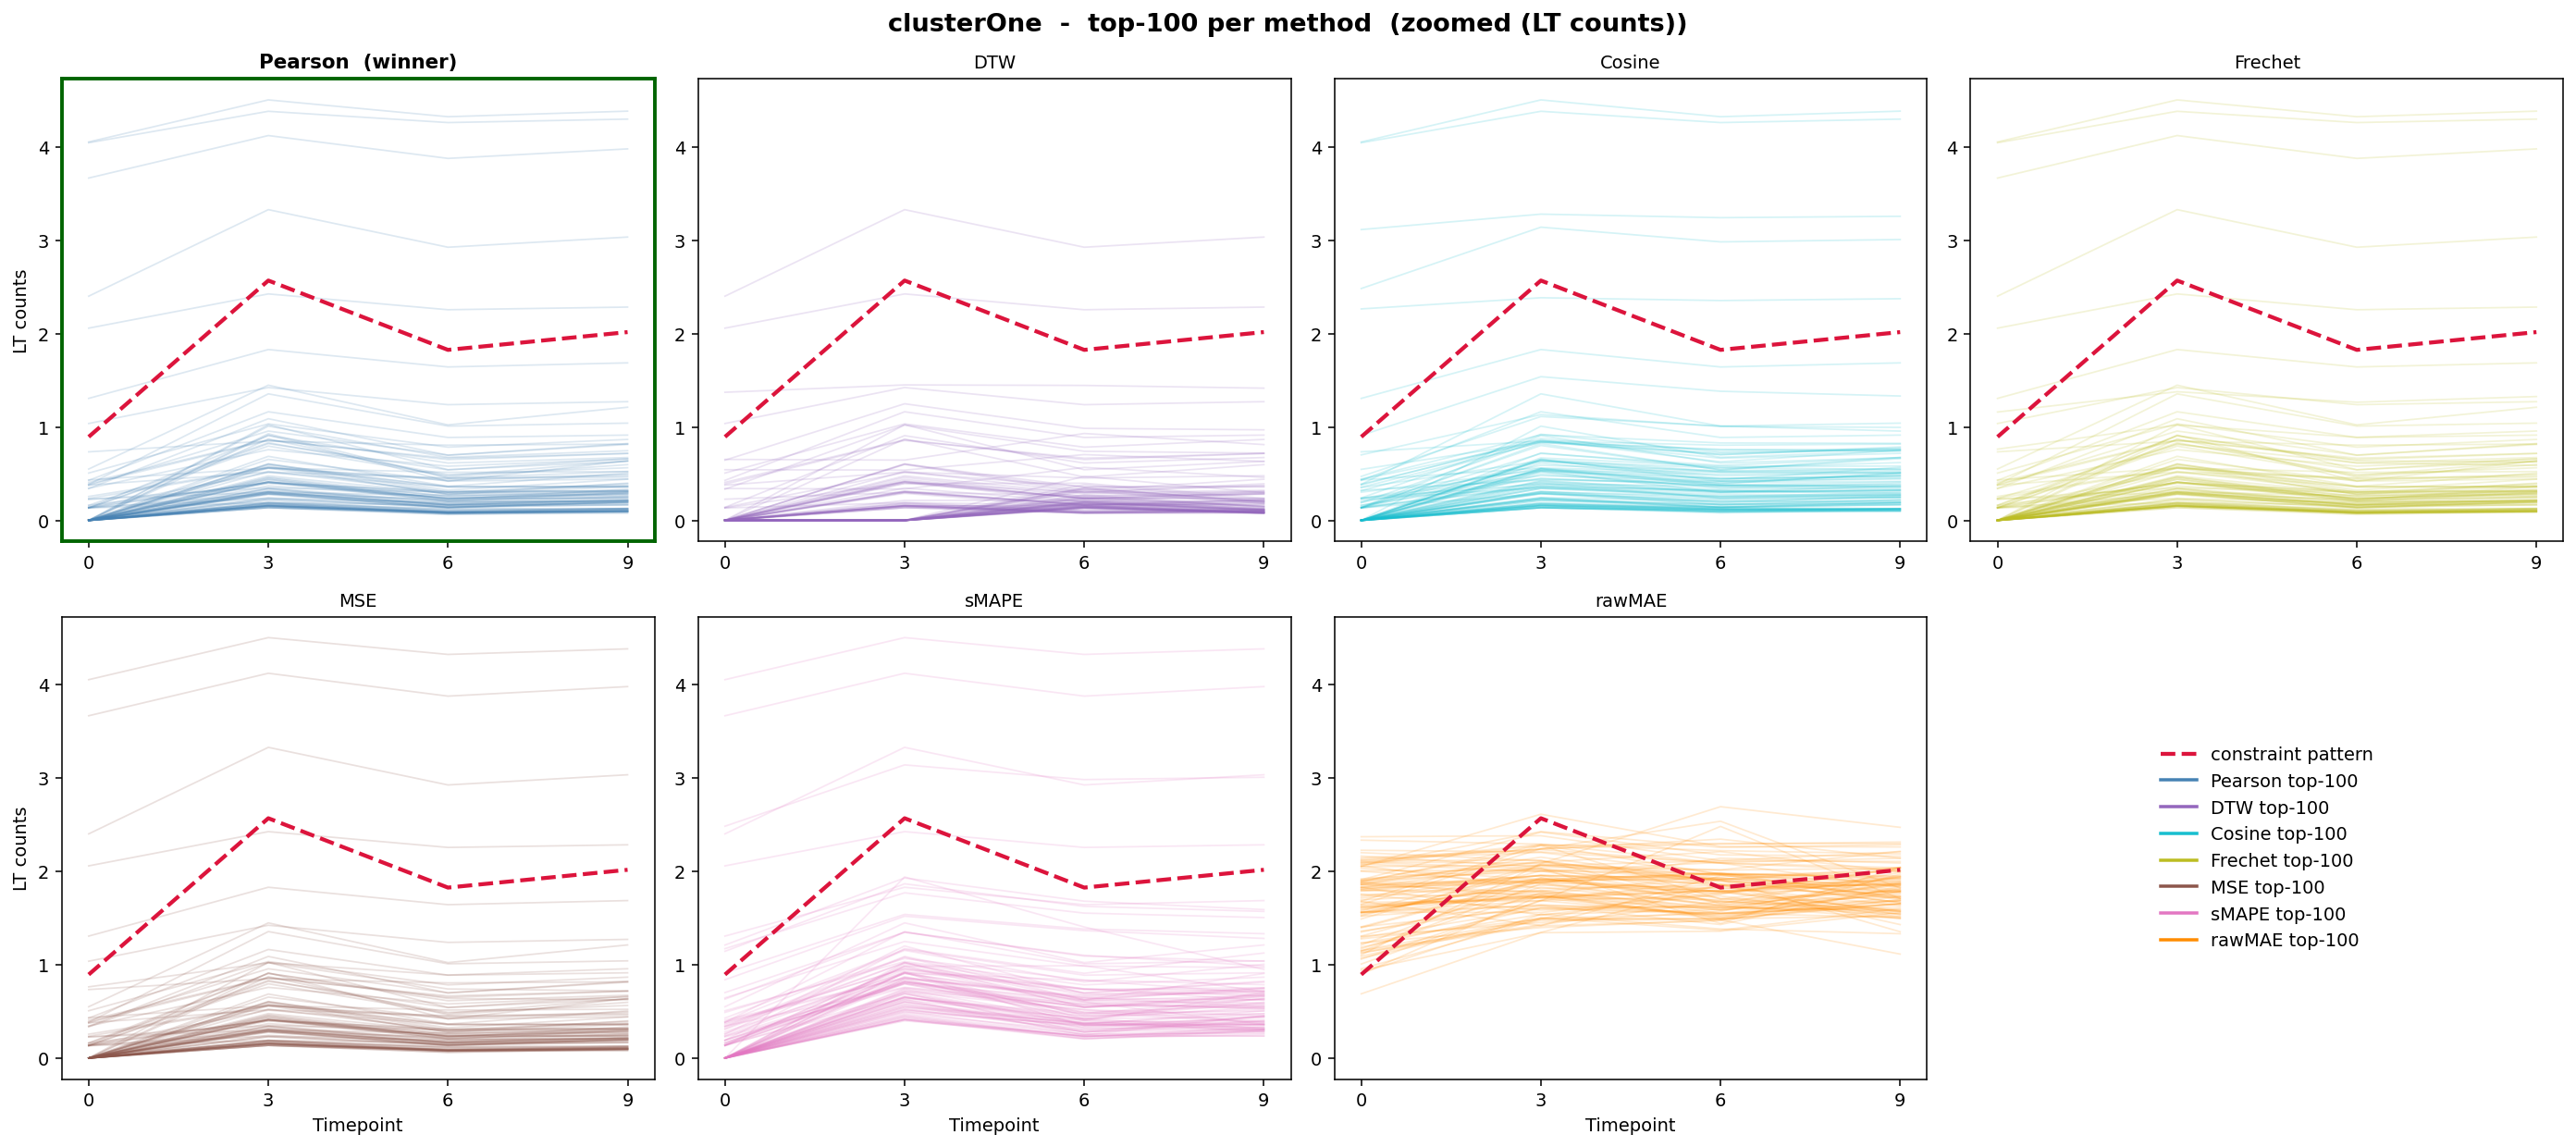
\includegraphics[height=0.83\textheight]{plots/gallery_top100_clusterOne_zoomed.png}
\end{frame}

\begin{frame}{clusterOne --- Top-100 per Method (Normalized)}
\centering
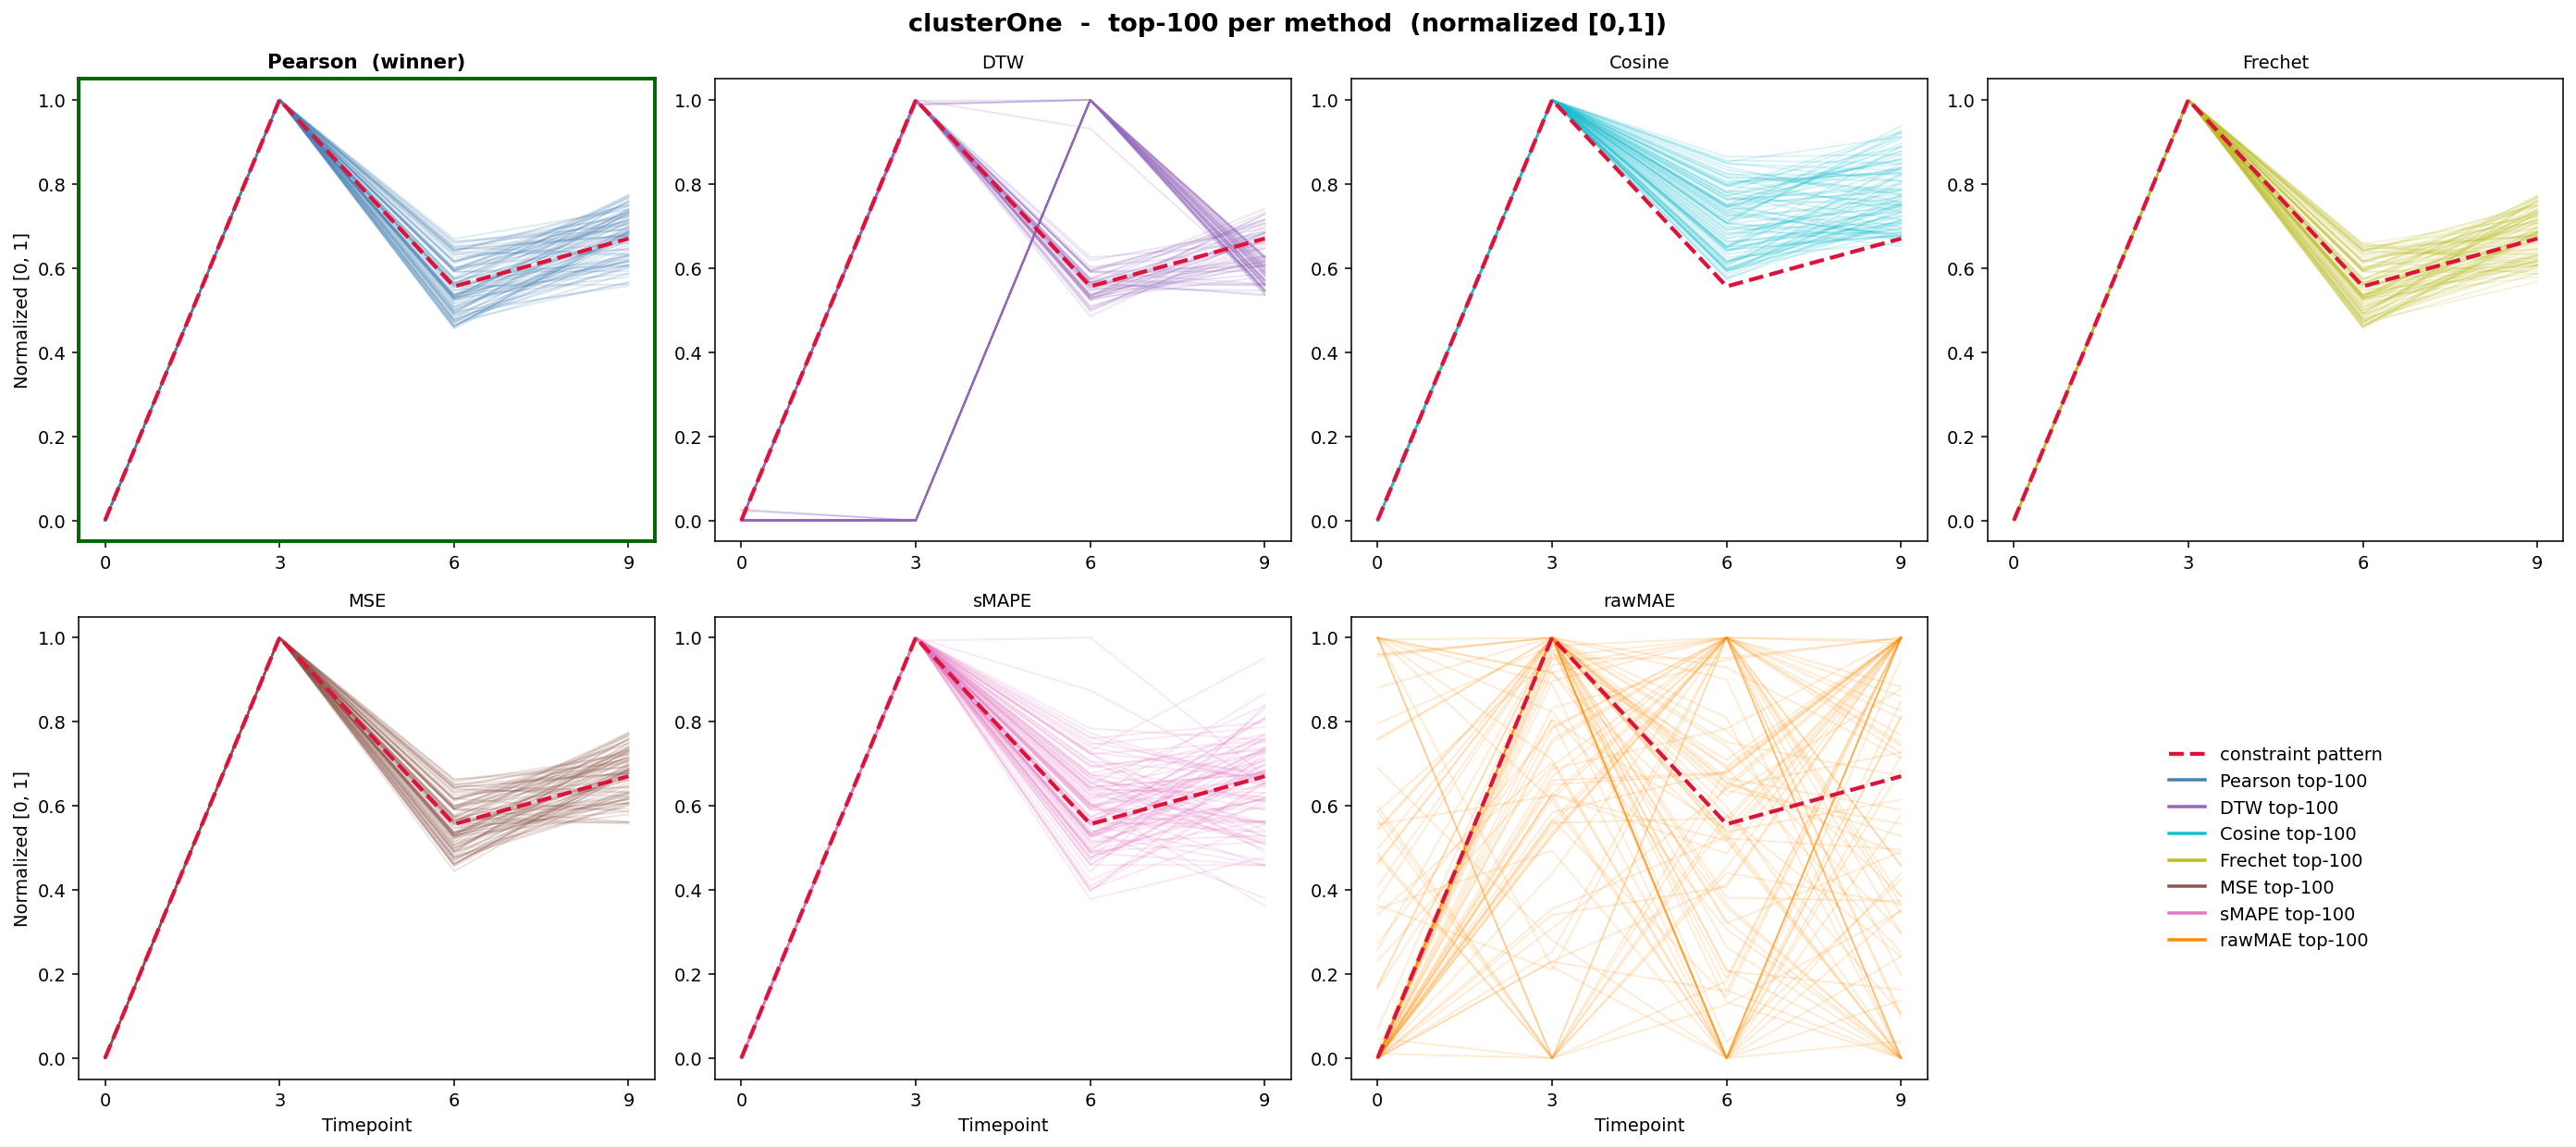
\includegraphics[height=0.83\textheight]{plots/gallery_top100_clusterOne_normalized.png}
\\[0.1em]
\scriptsize Pearson, Fr\'{e}chet, MSE: clean shape overlays. DTW, Cosine, sMAPE: visible shape variance. rawMAE: chaos --- magnitude-correct picks fail the shape test.
\end{frame}

\begin{frame}{clusterOne --- Top-100 per Method (Mean-Shifted)}
\centering
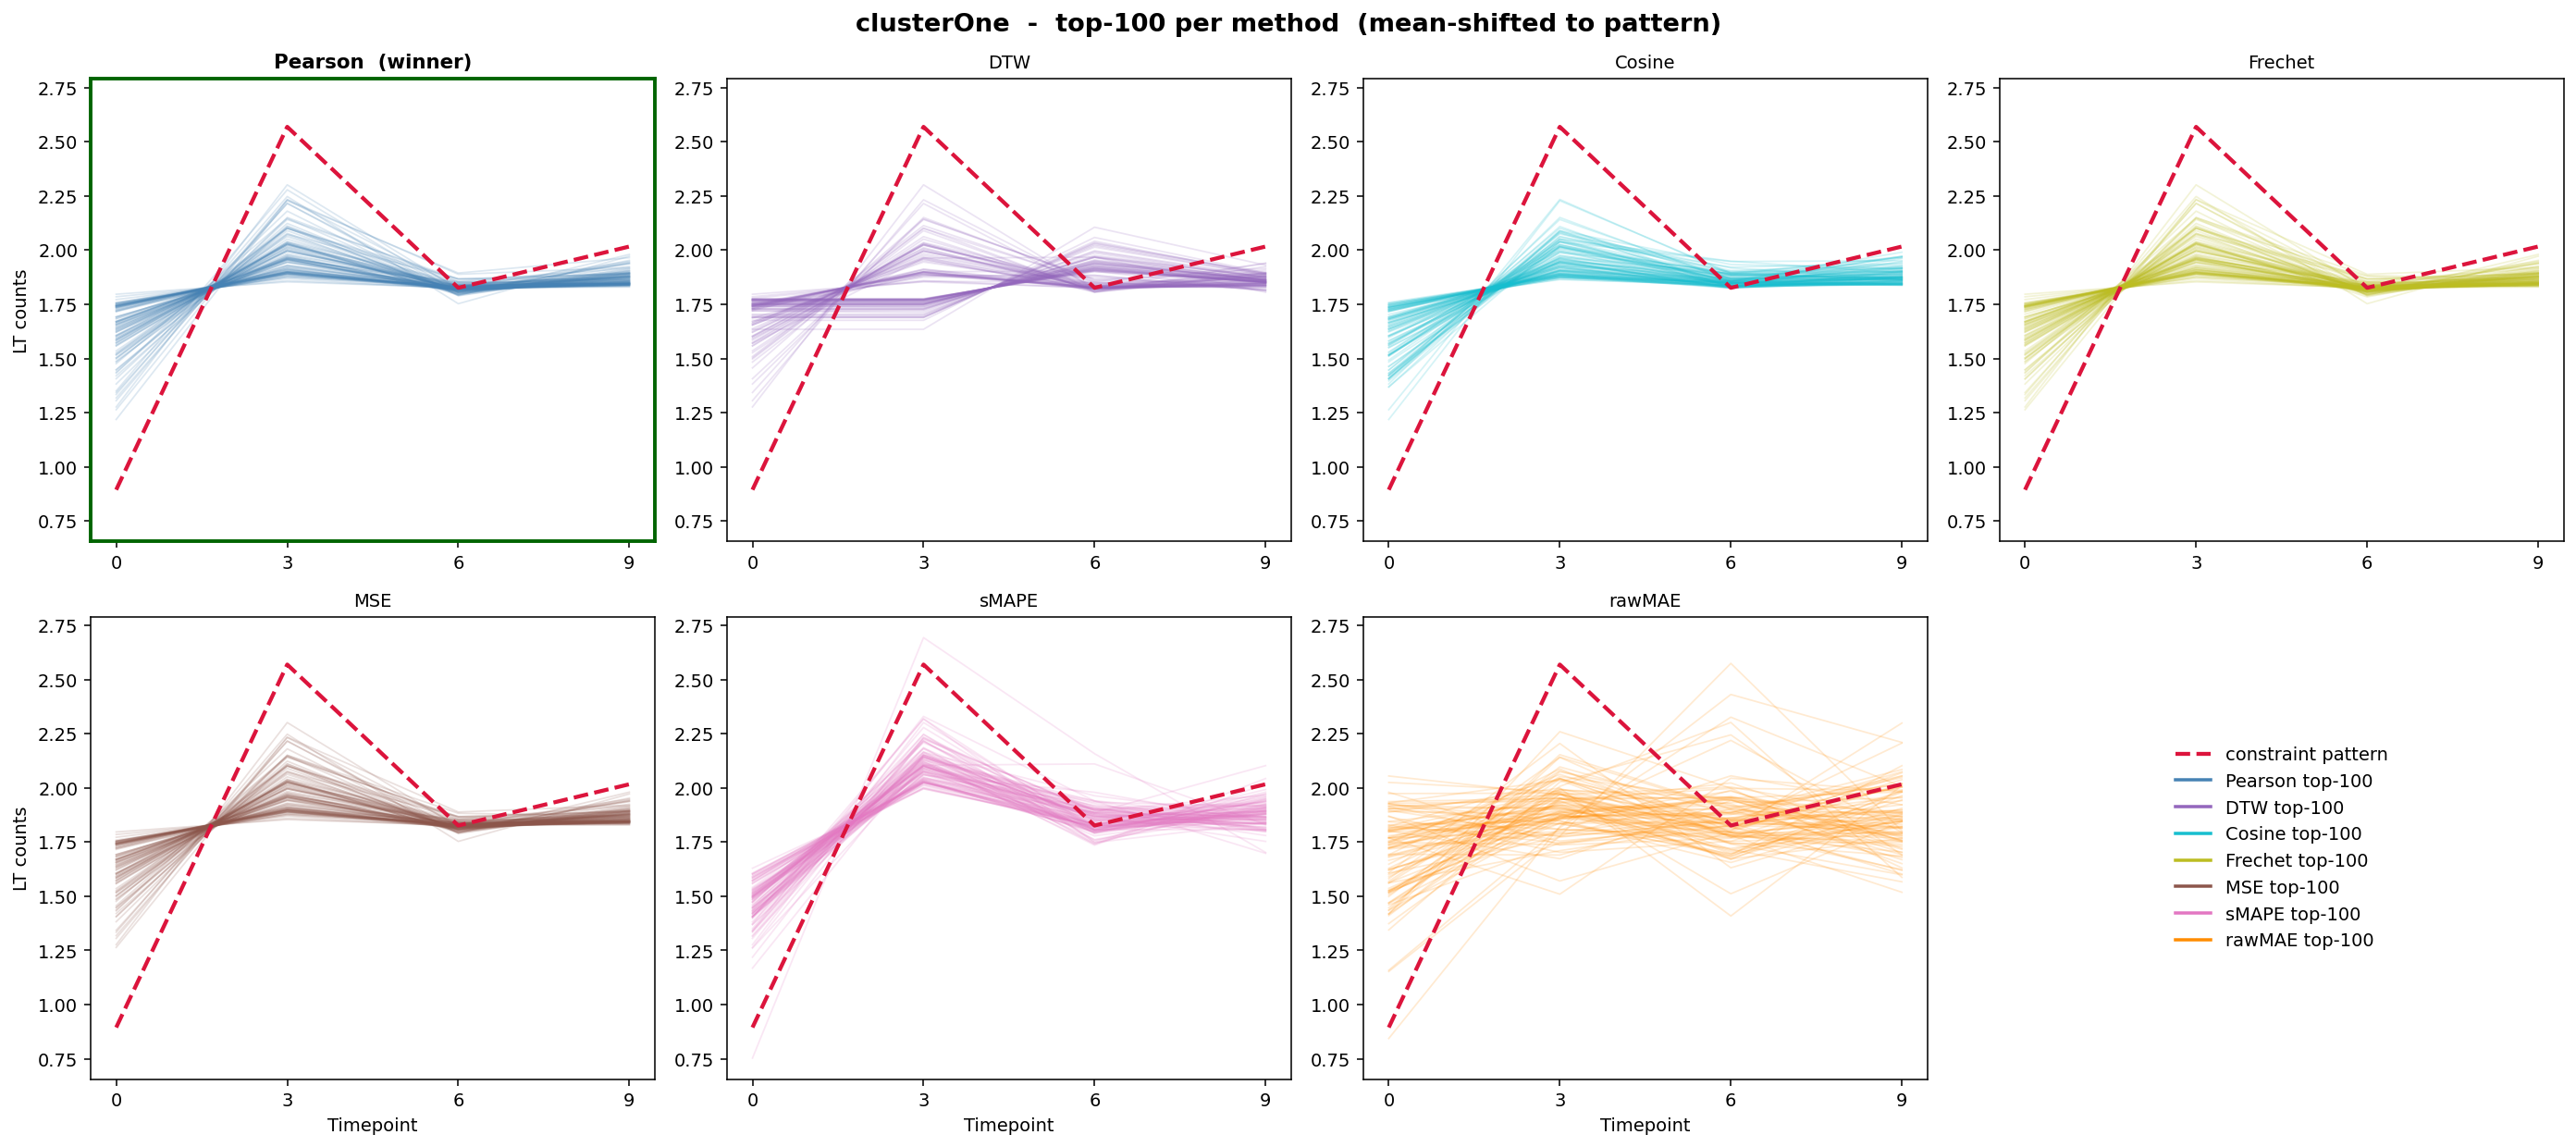
\includegraphics[height=0.83\textheight]{plots/gallery_top100_clusterOne_meanshift.png}
\\[0.1em]
\scriptsize Each gene additively shifted to the pattern's mean (removes the magnitude excuse, forces a pure-shape view). Pearson and the consensus group trace the up-down-up; rawMAE genes are still chaos when shifted.
\end{frame}

% ==================================================================
% clusterTwo
% ==================================================================
\begin{frame}{clusterTwo --- Top-100 per Method (Zoomed)}
\centering
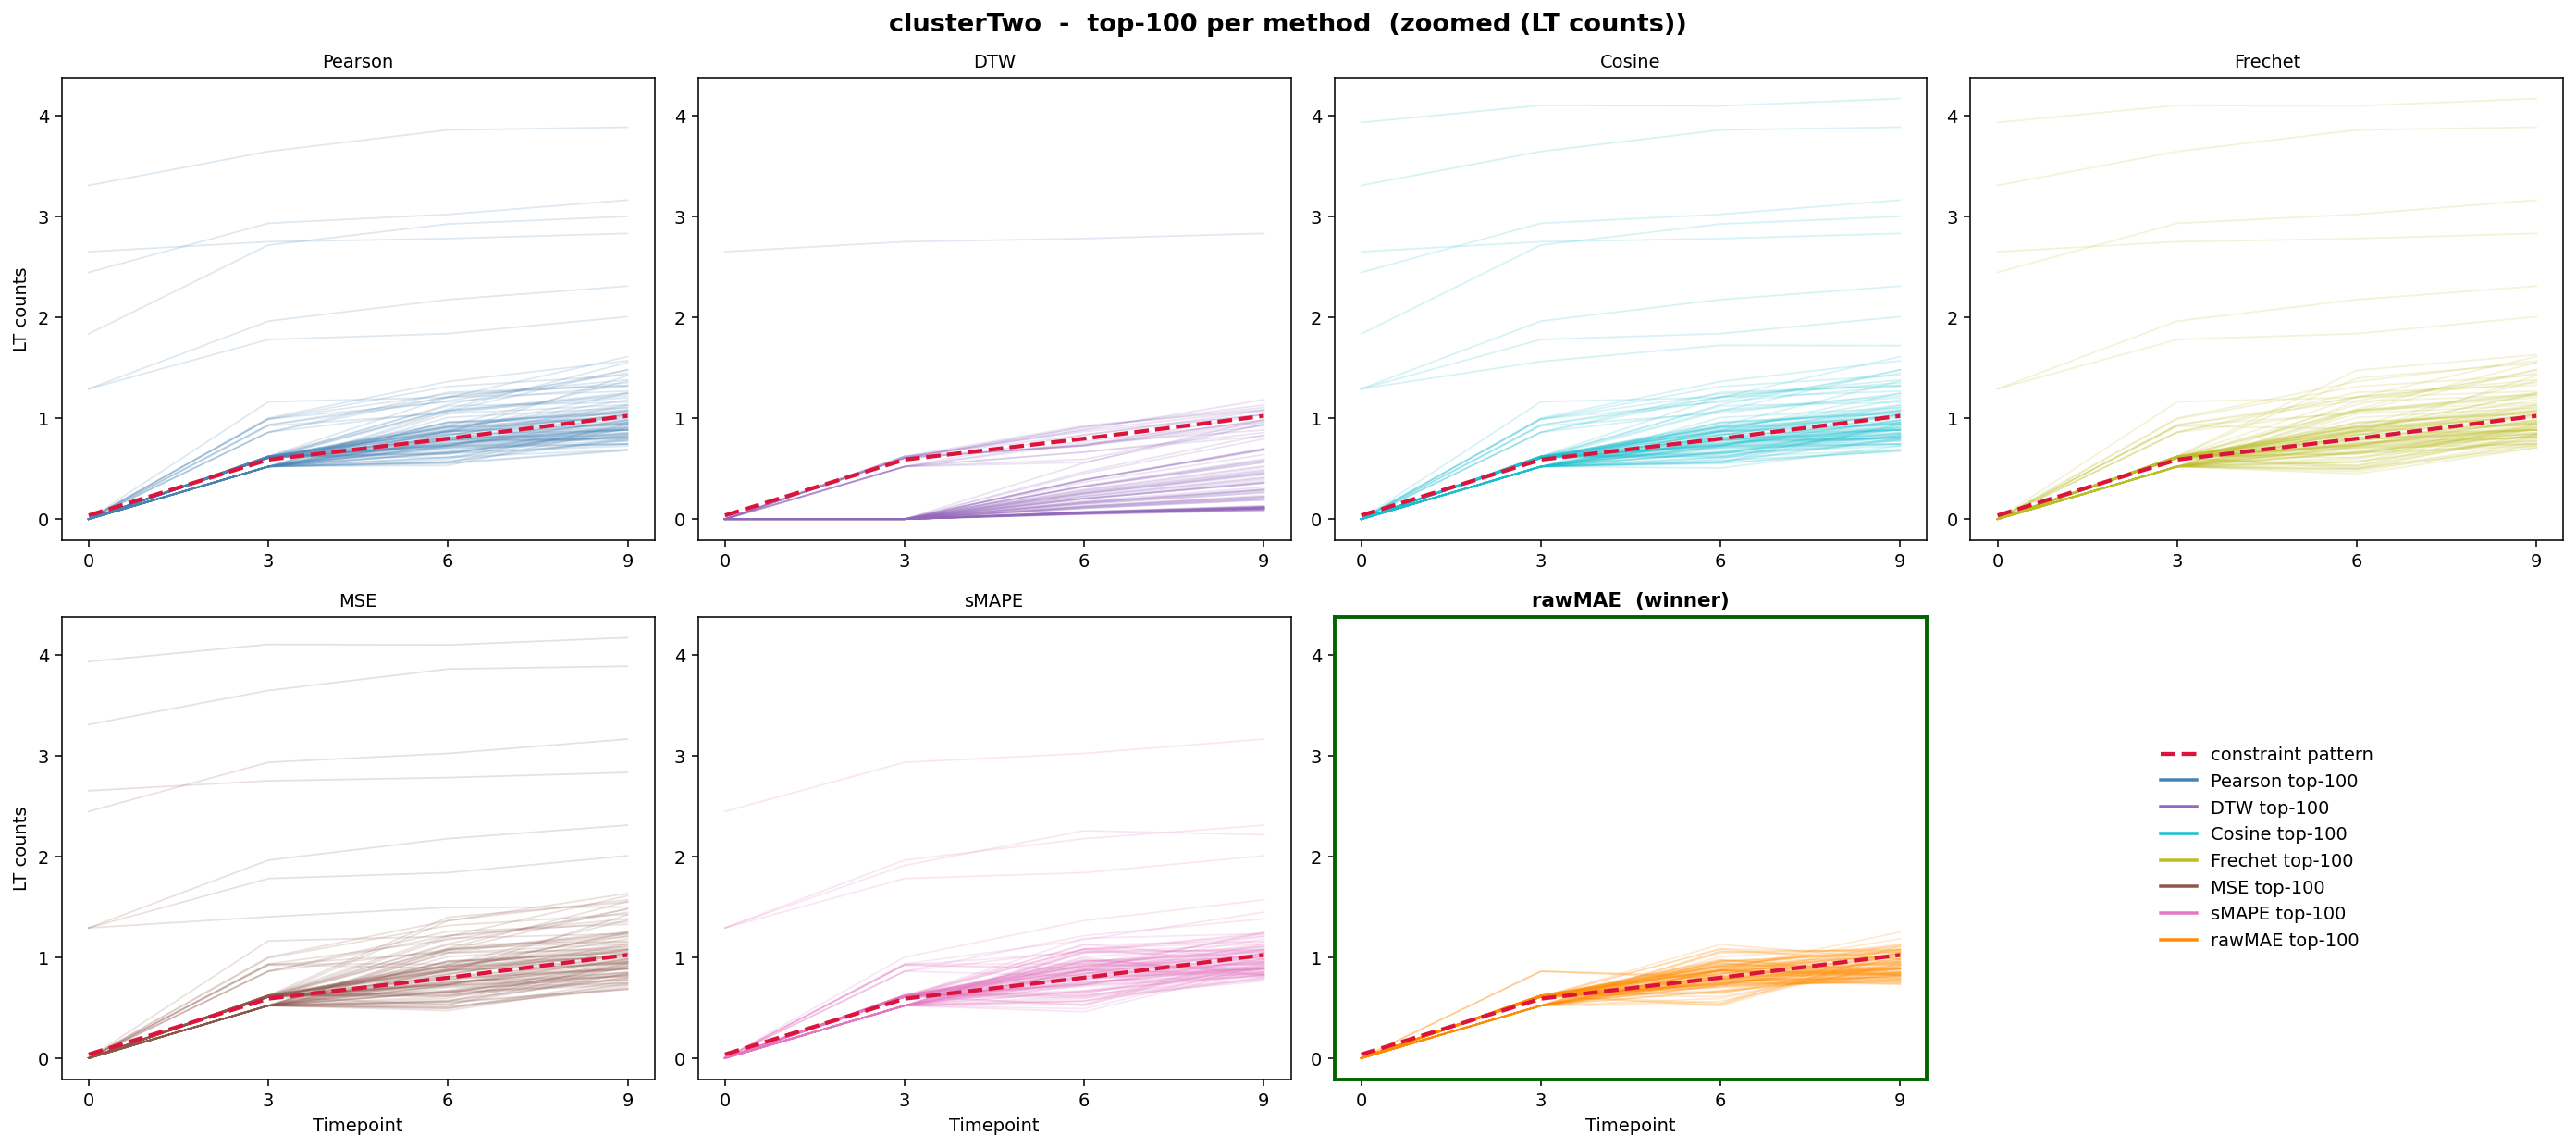
\includegraphics[height=0.83\textheight]{plots/gallery_top100_clusterTwo_zoomed.png}
\\[0.1em]
\scriptsize rawMAE picks hug the monotone-increase pattern at its actual amplitude. The shape-only methods pick genes with the right shape but spreading up to LT $\sim$4.
\end{frame}

\begin{frame}{clusterTwo --- Top-100 per Method (Normalized)}
\centering
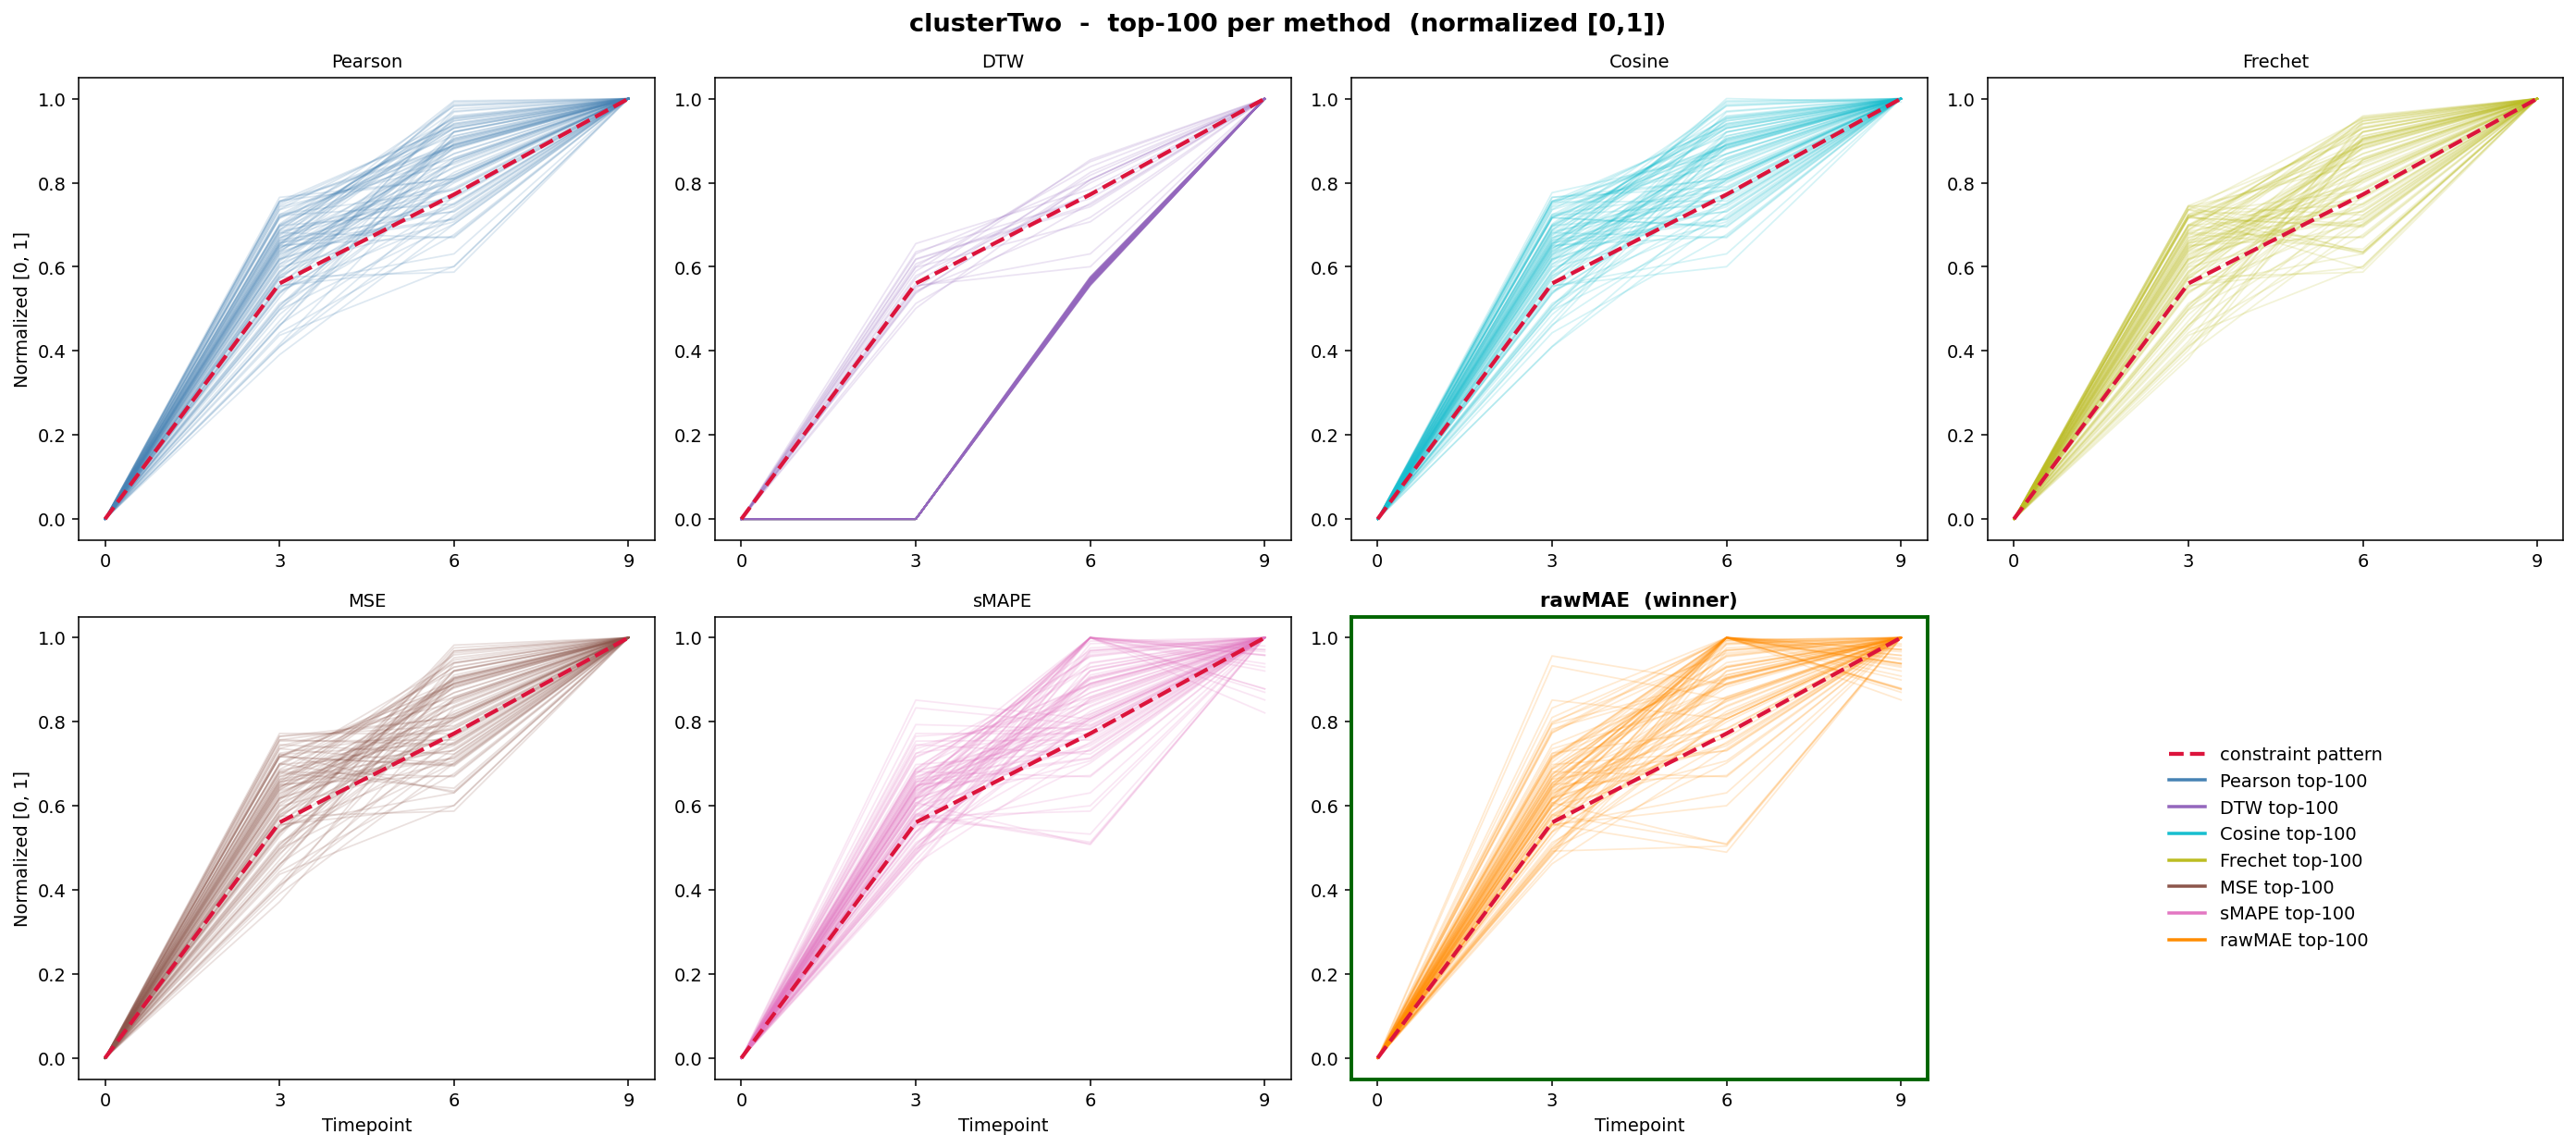
\includegraphics[height=0.83\textheight]{plots/gallery_top100_clusterTwo_normalized.png}
\\[0.1em]
\scriptsize After normalization, all methods look similar --- their shape picks are roughly the same. The differentiation is in magnitude (zoomed view).
\end{frame}

% ==================================================================
% clusterThree
% ==================================================================
\begin{frame}{clusterThree --- Top-100 per Method (Zoomed)}
\centering
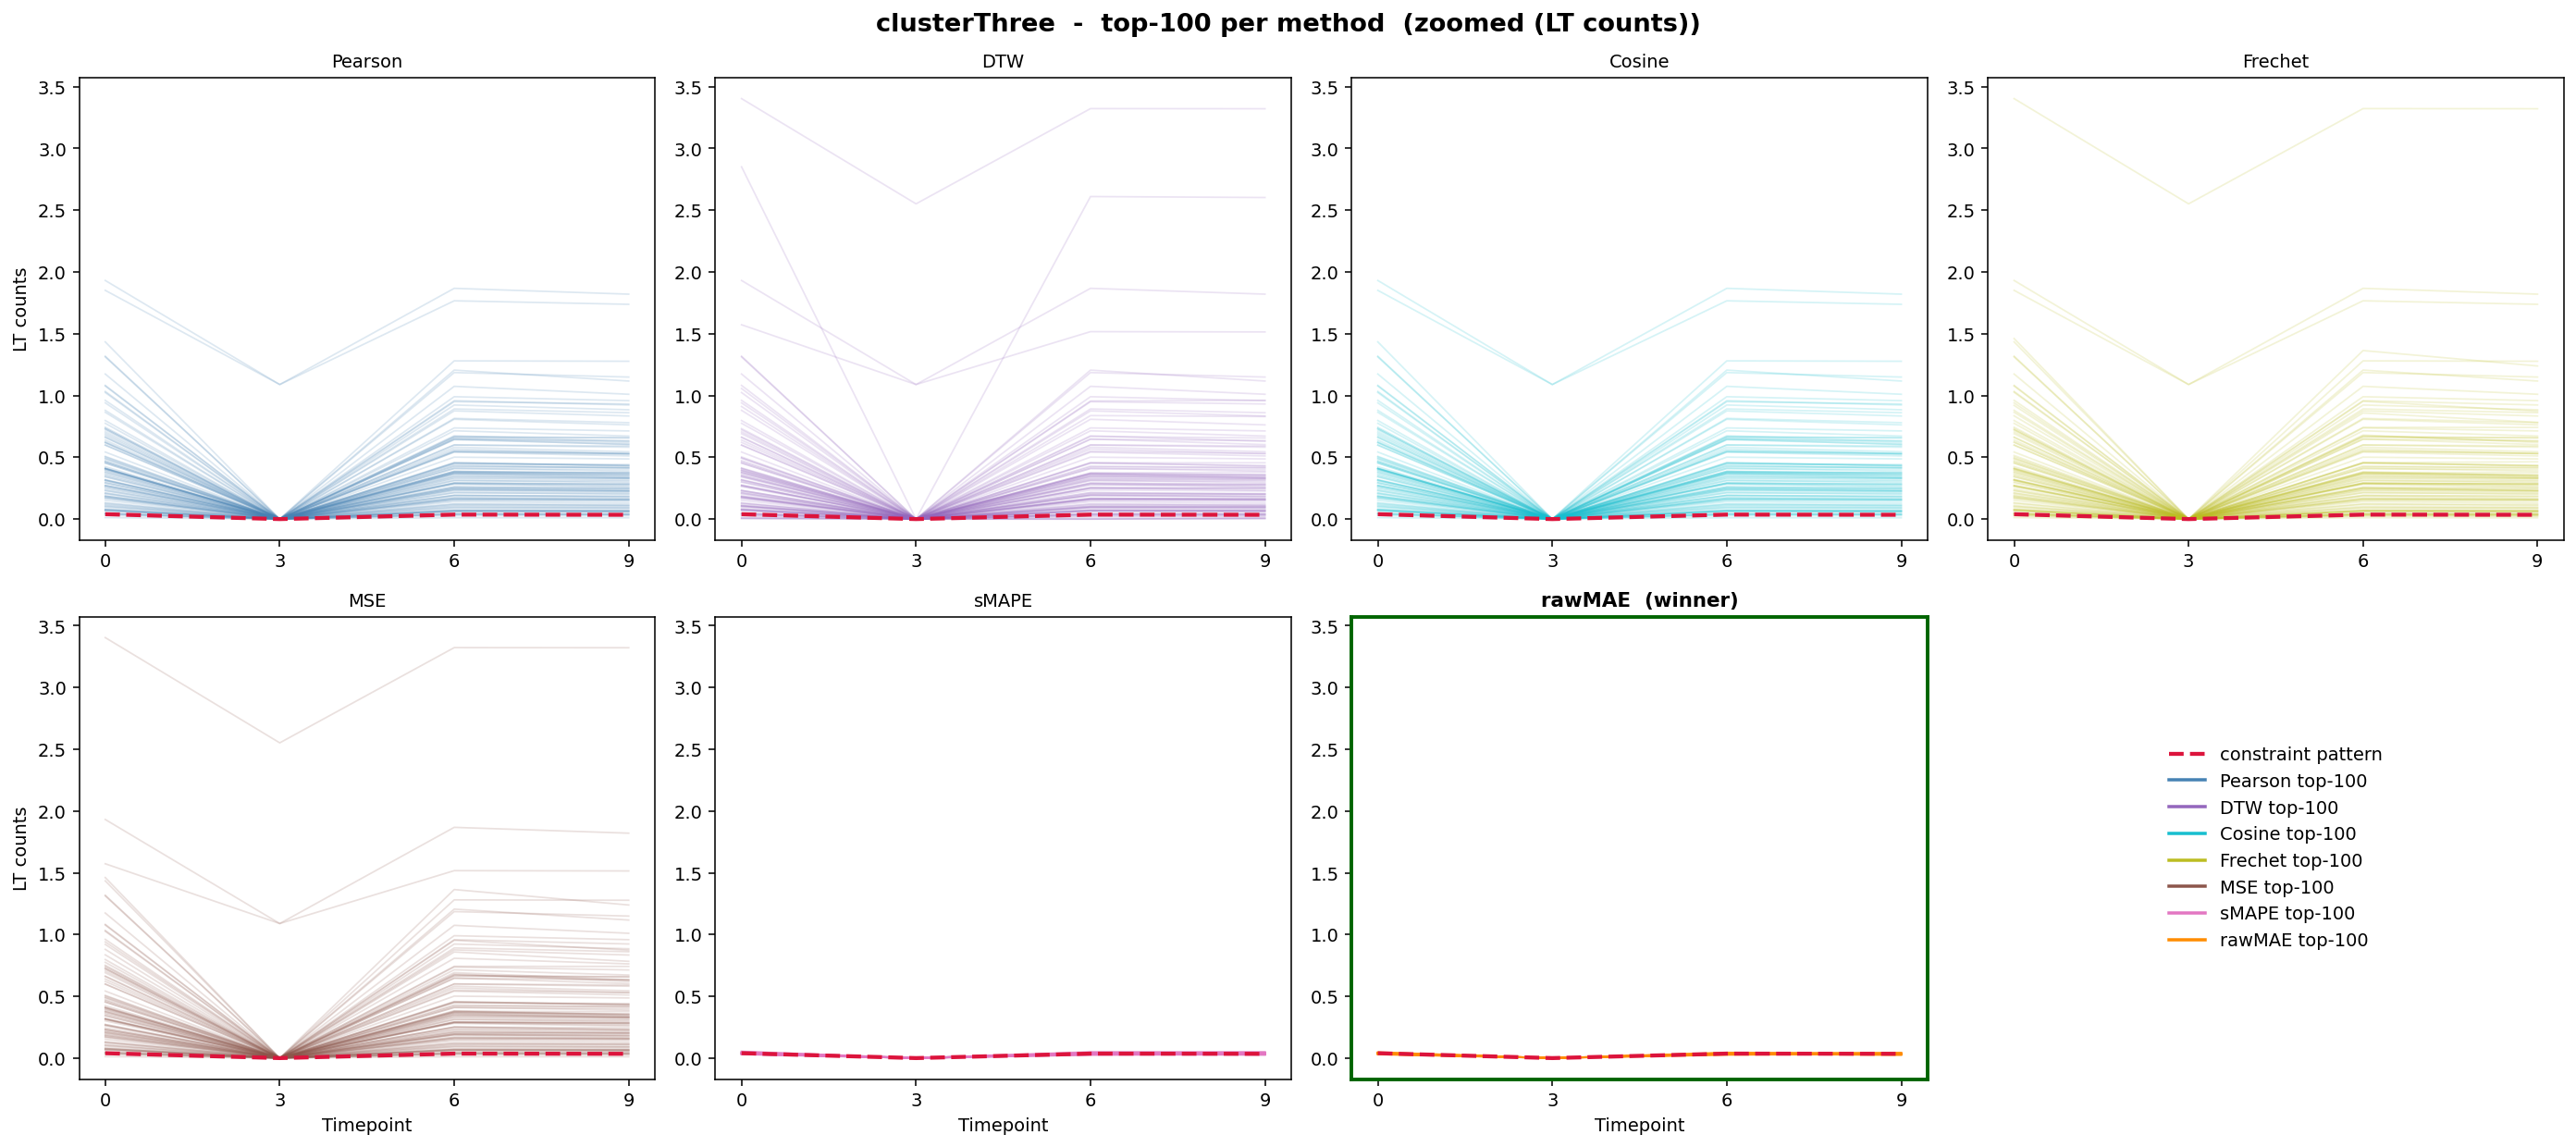
\includegraphics[height=0.83\textheight]{plots/gallery_top100_clusterThree_zoomed.png}
\\[0.1em]
\scriptsize rawMAE picks live on the V-shape at the pattern's tiny magnitude (range $\sim$0.04). Shape methods pick genes 5--40$\times$ above the pattern's range.
\end{frame}

\begin{frame}{clusterThree --- Top-100 per Method (Normalized)}
\centering
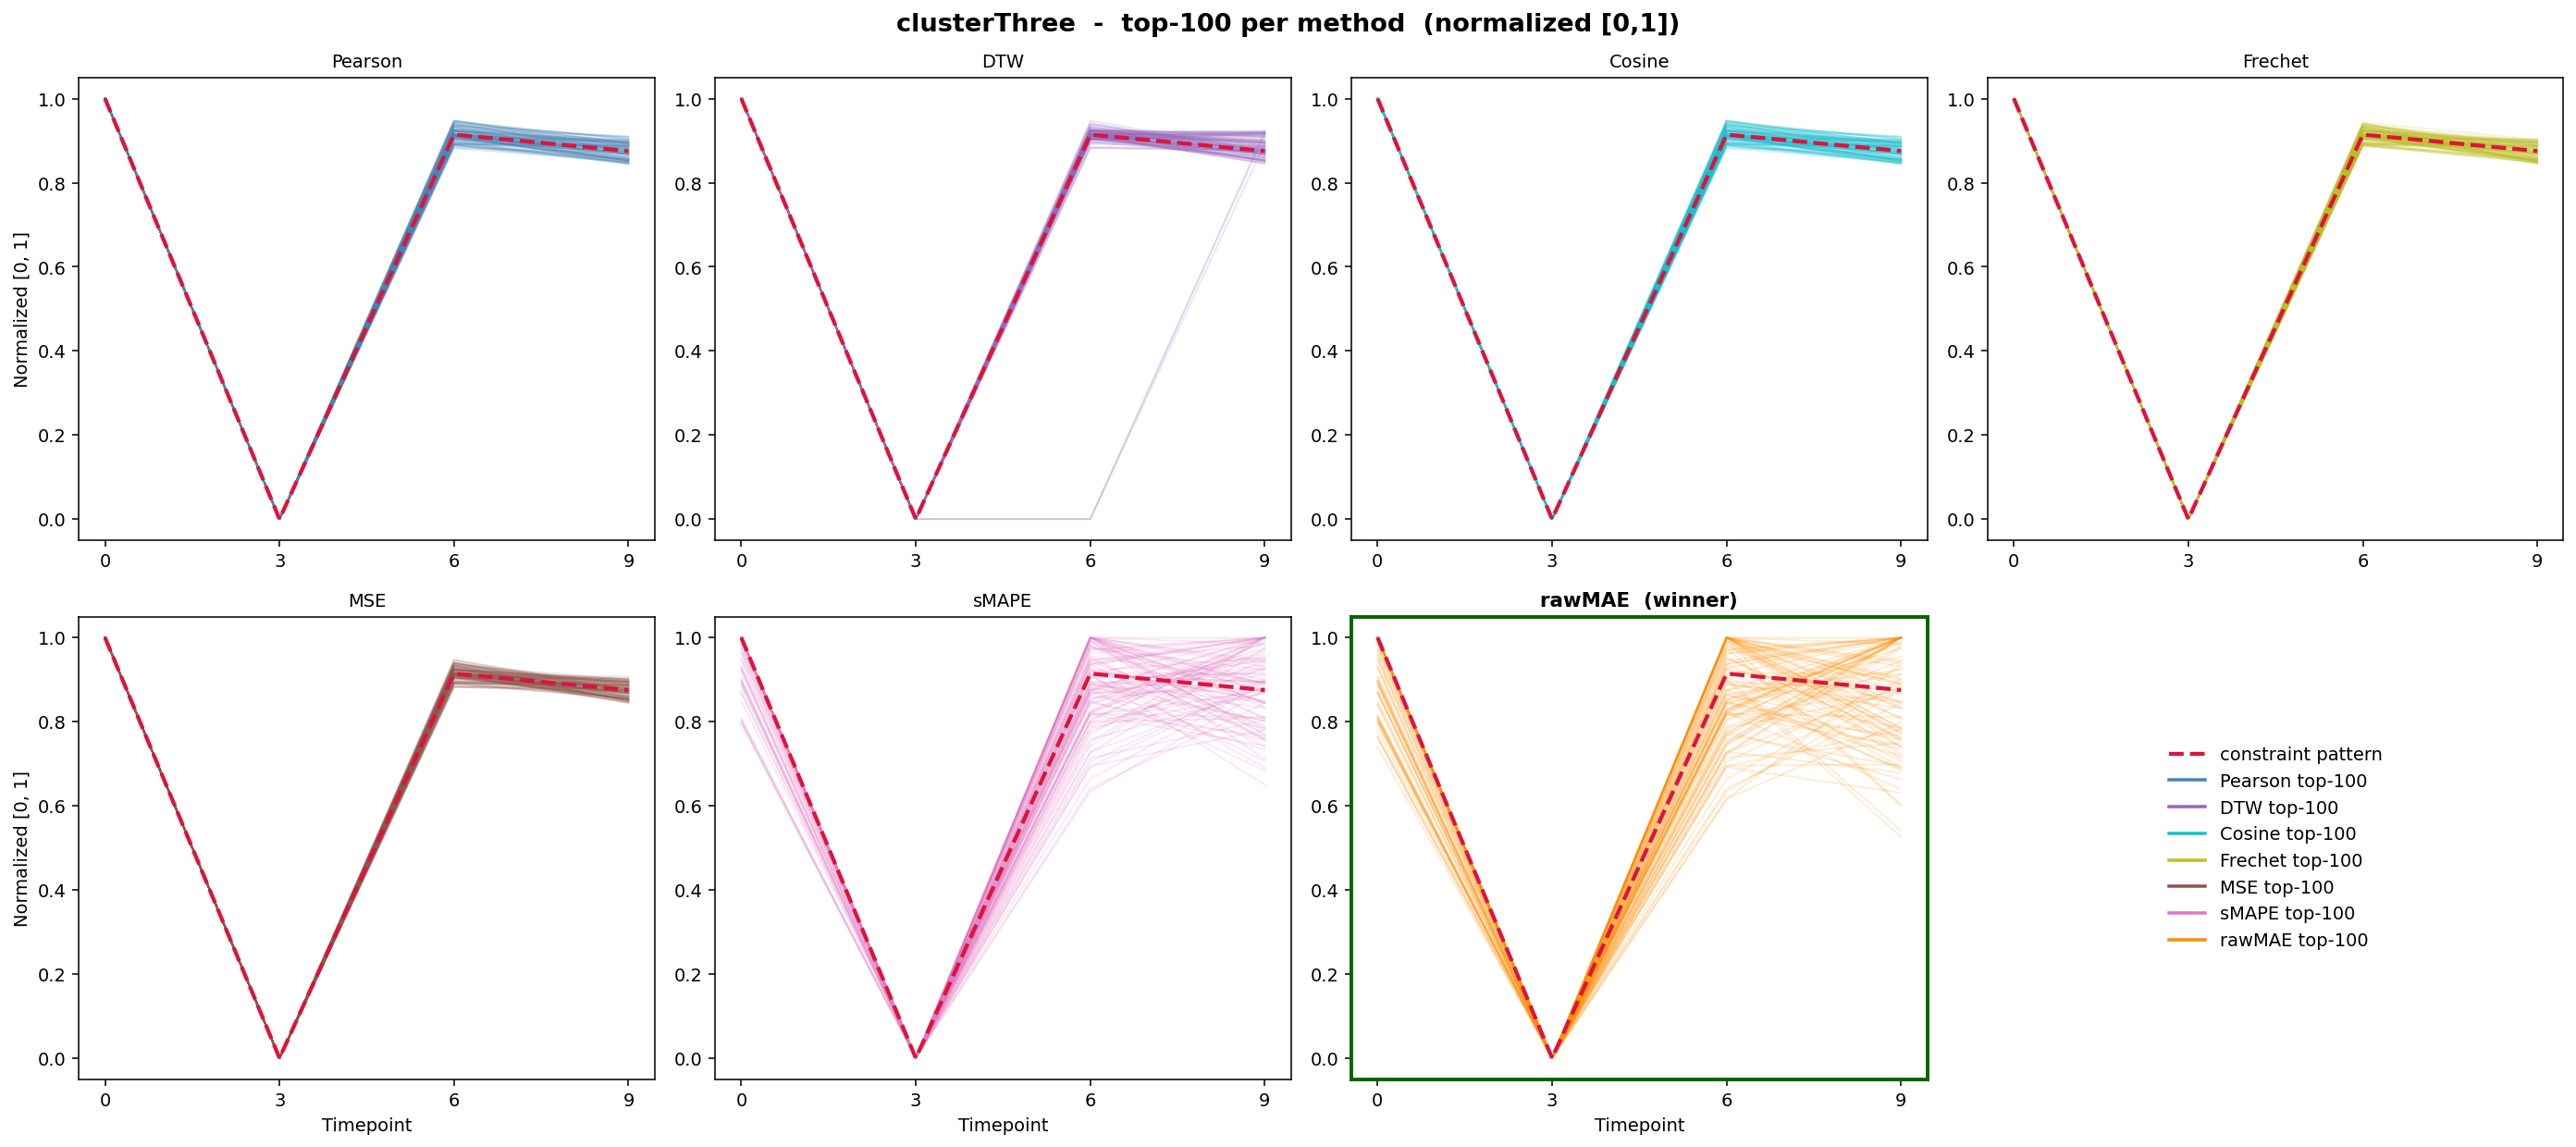
\includegraphics[height=0.83\textheight]{plots/gallery_top100_clusterThree_normalized.png}
\\[0.1em]
\scriptsize Normalized: most methods recover the V-shape. Magnitude (zoomed) is the differentiator.
\end{frame}

% ==================================================================
% clusterFour
% ==================================================================
\begin{frame}{clusterFour --- Top-100 per Method (Zoomed)}
\centering
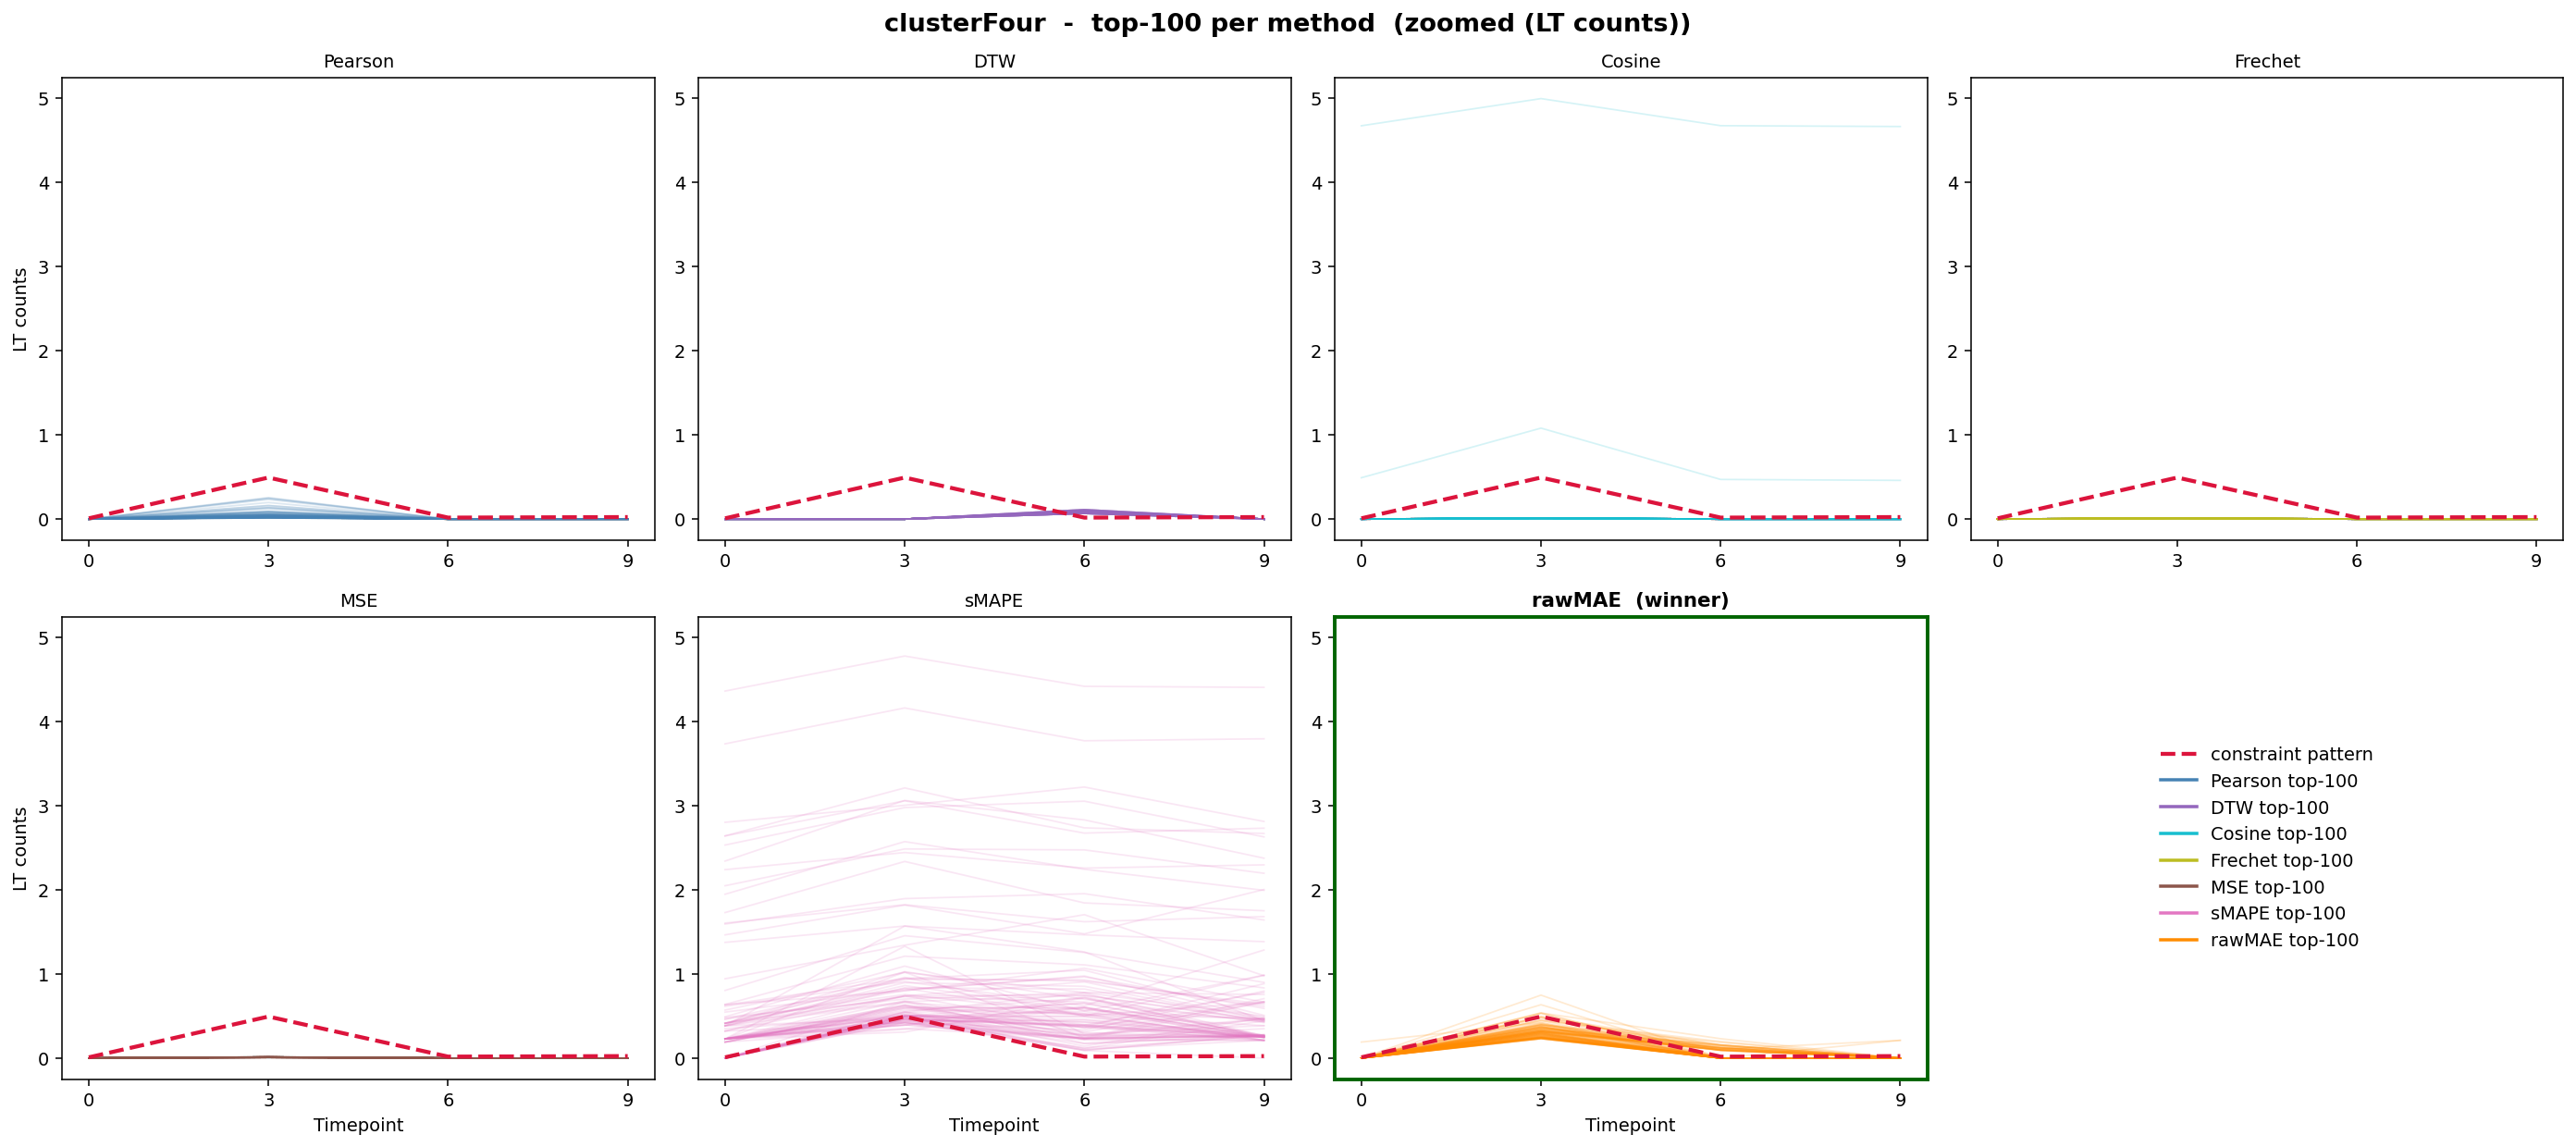
\includegraphics[height=0.83\textheight]{plots/gallery_top100_clusterFour_zoomed.png}
\\[0.1em]
\scriptsize rawMAE captures the $t{=}3$ spike. Shape methods pick flat-ish genes --- normalization erased the spike upstream. DTW picks anti-correlated genes ($r_{\mathrm{med}} = -0.33$).
\end{frame}

\begin{frame}{clusterFour --- Top-100 per Method (Normalized)}
\centering
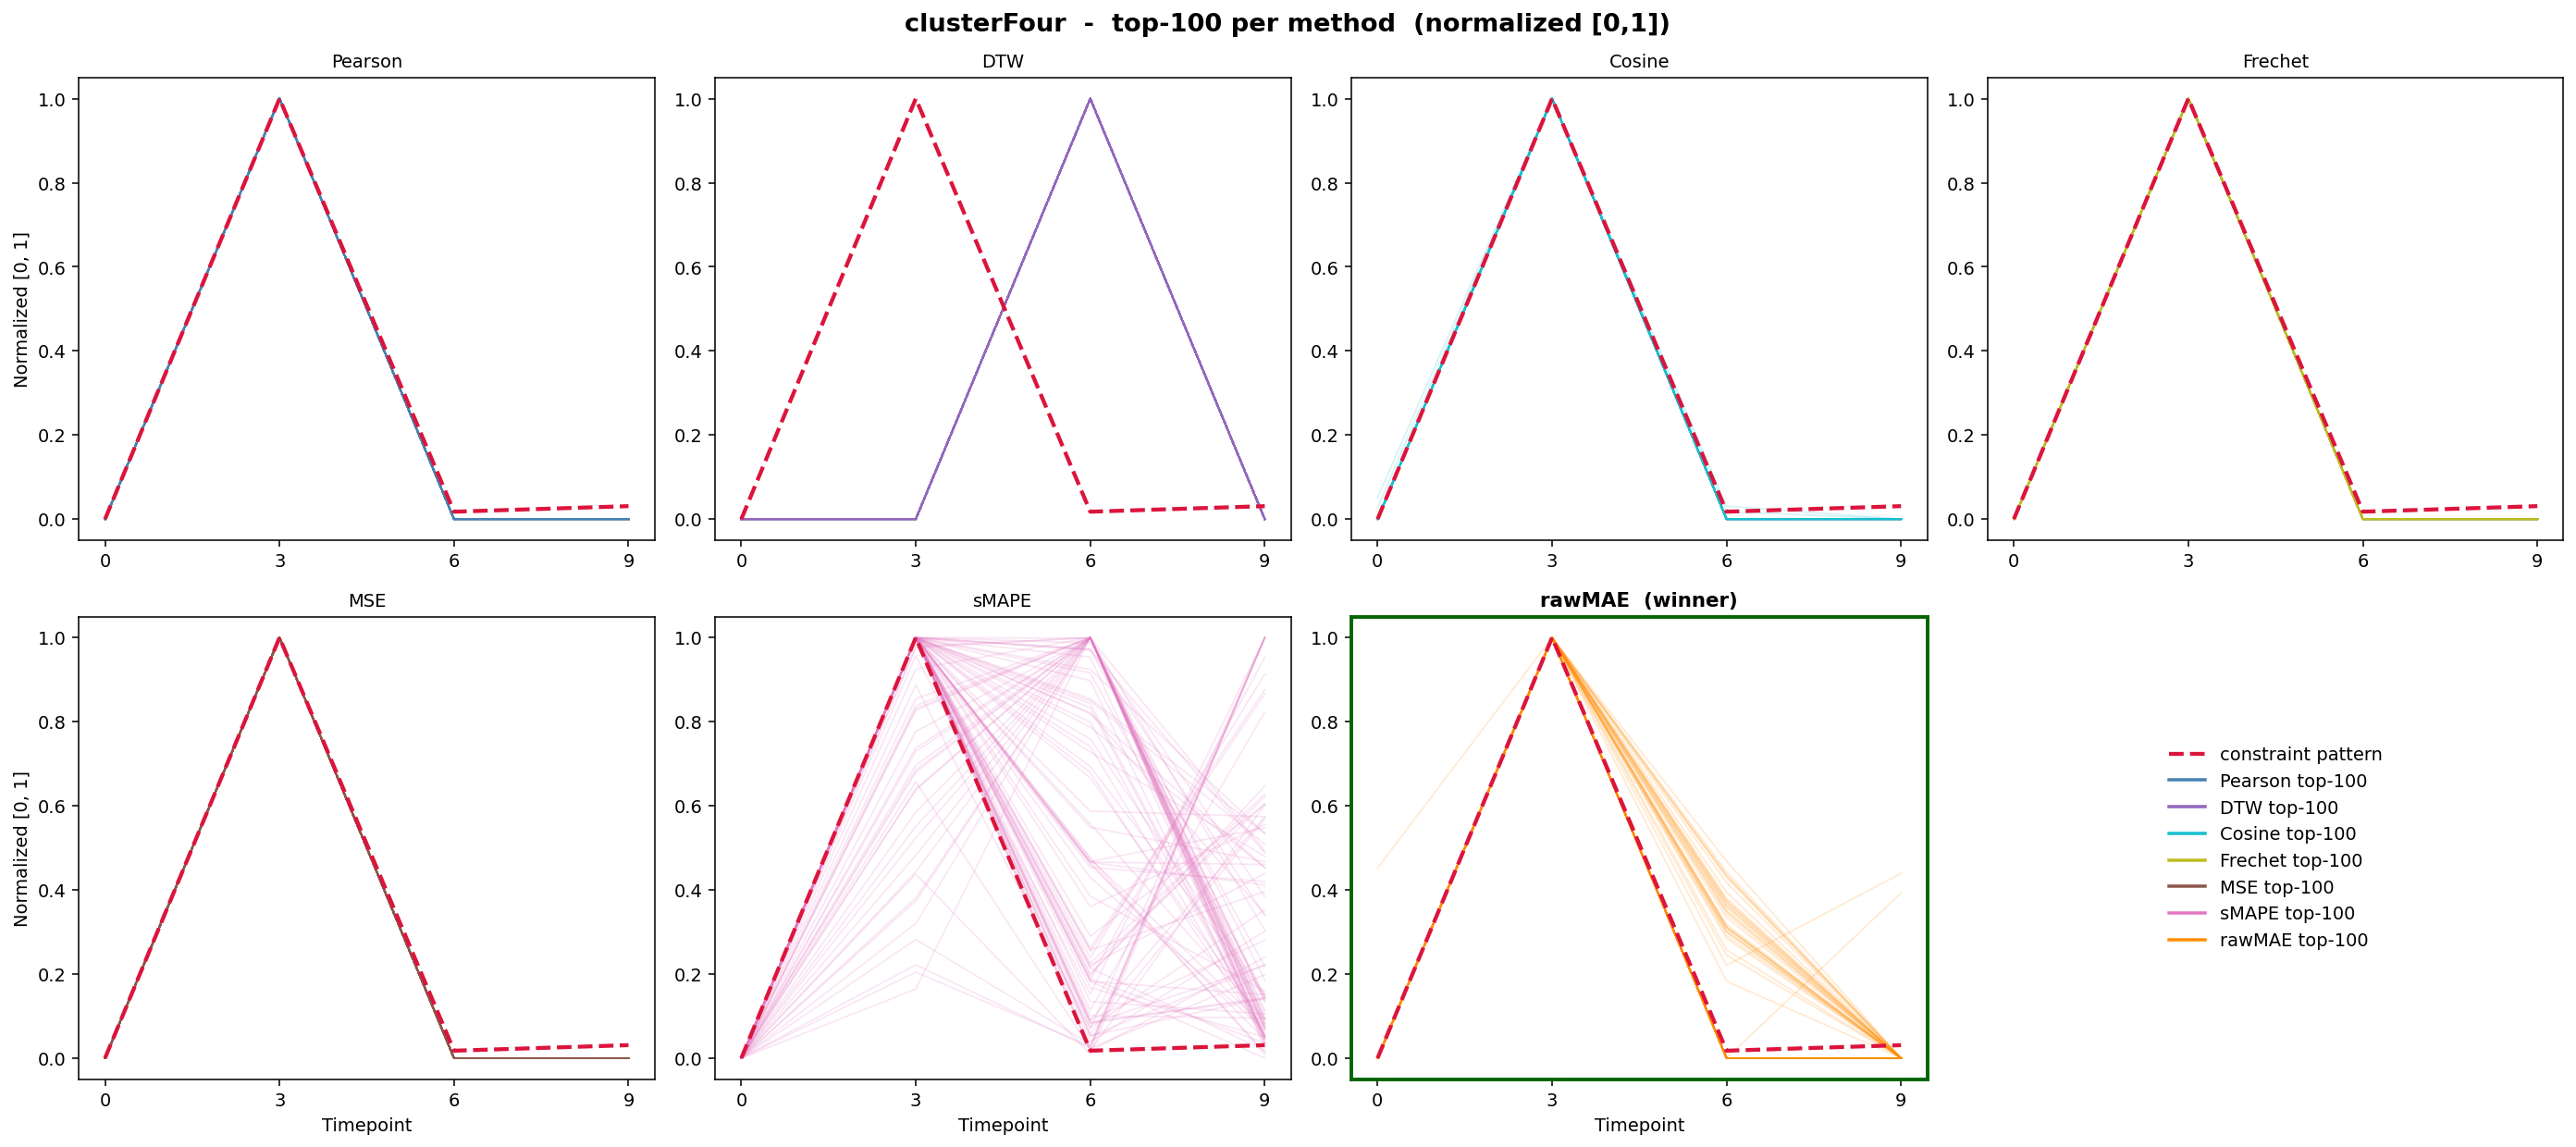
\includegraphics[height=0.83\textheight]{plots/gallery_top100_clusterFour_normalized.png}
\\[0.1em]
\scriptsize Normalized: rawMAE and most shape methods recover the spike. DTW noticeably picks anti-correlated genes.
\end{frame}

% ------------------------------------------------------------------
\begin{frame}{Top-100 Overlap Across Methods}
\centering
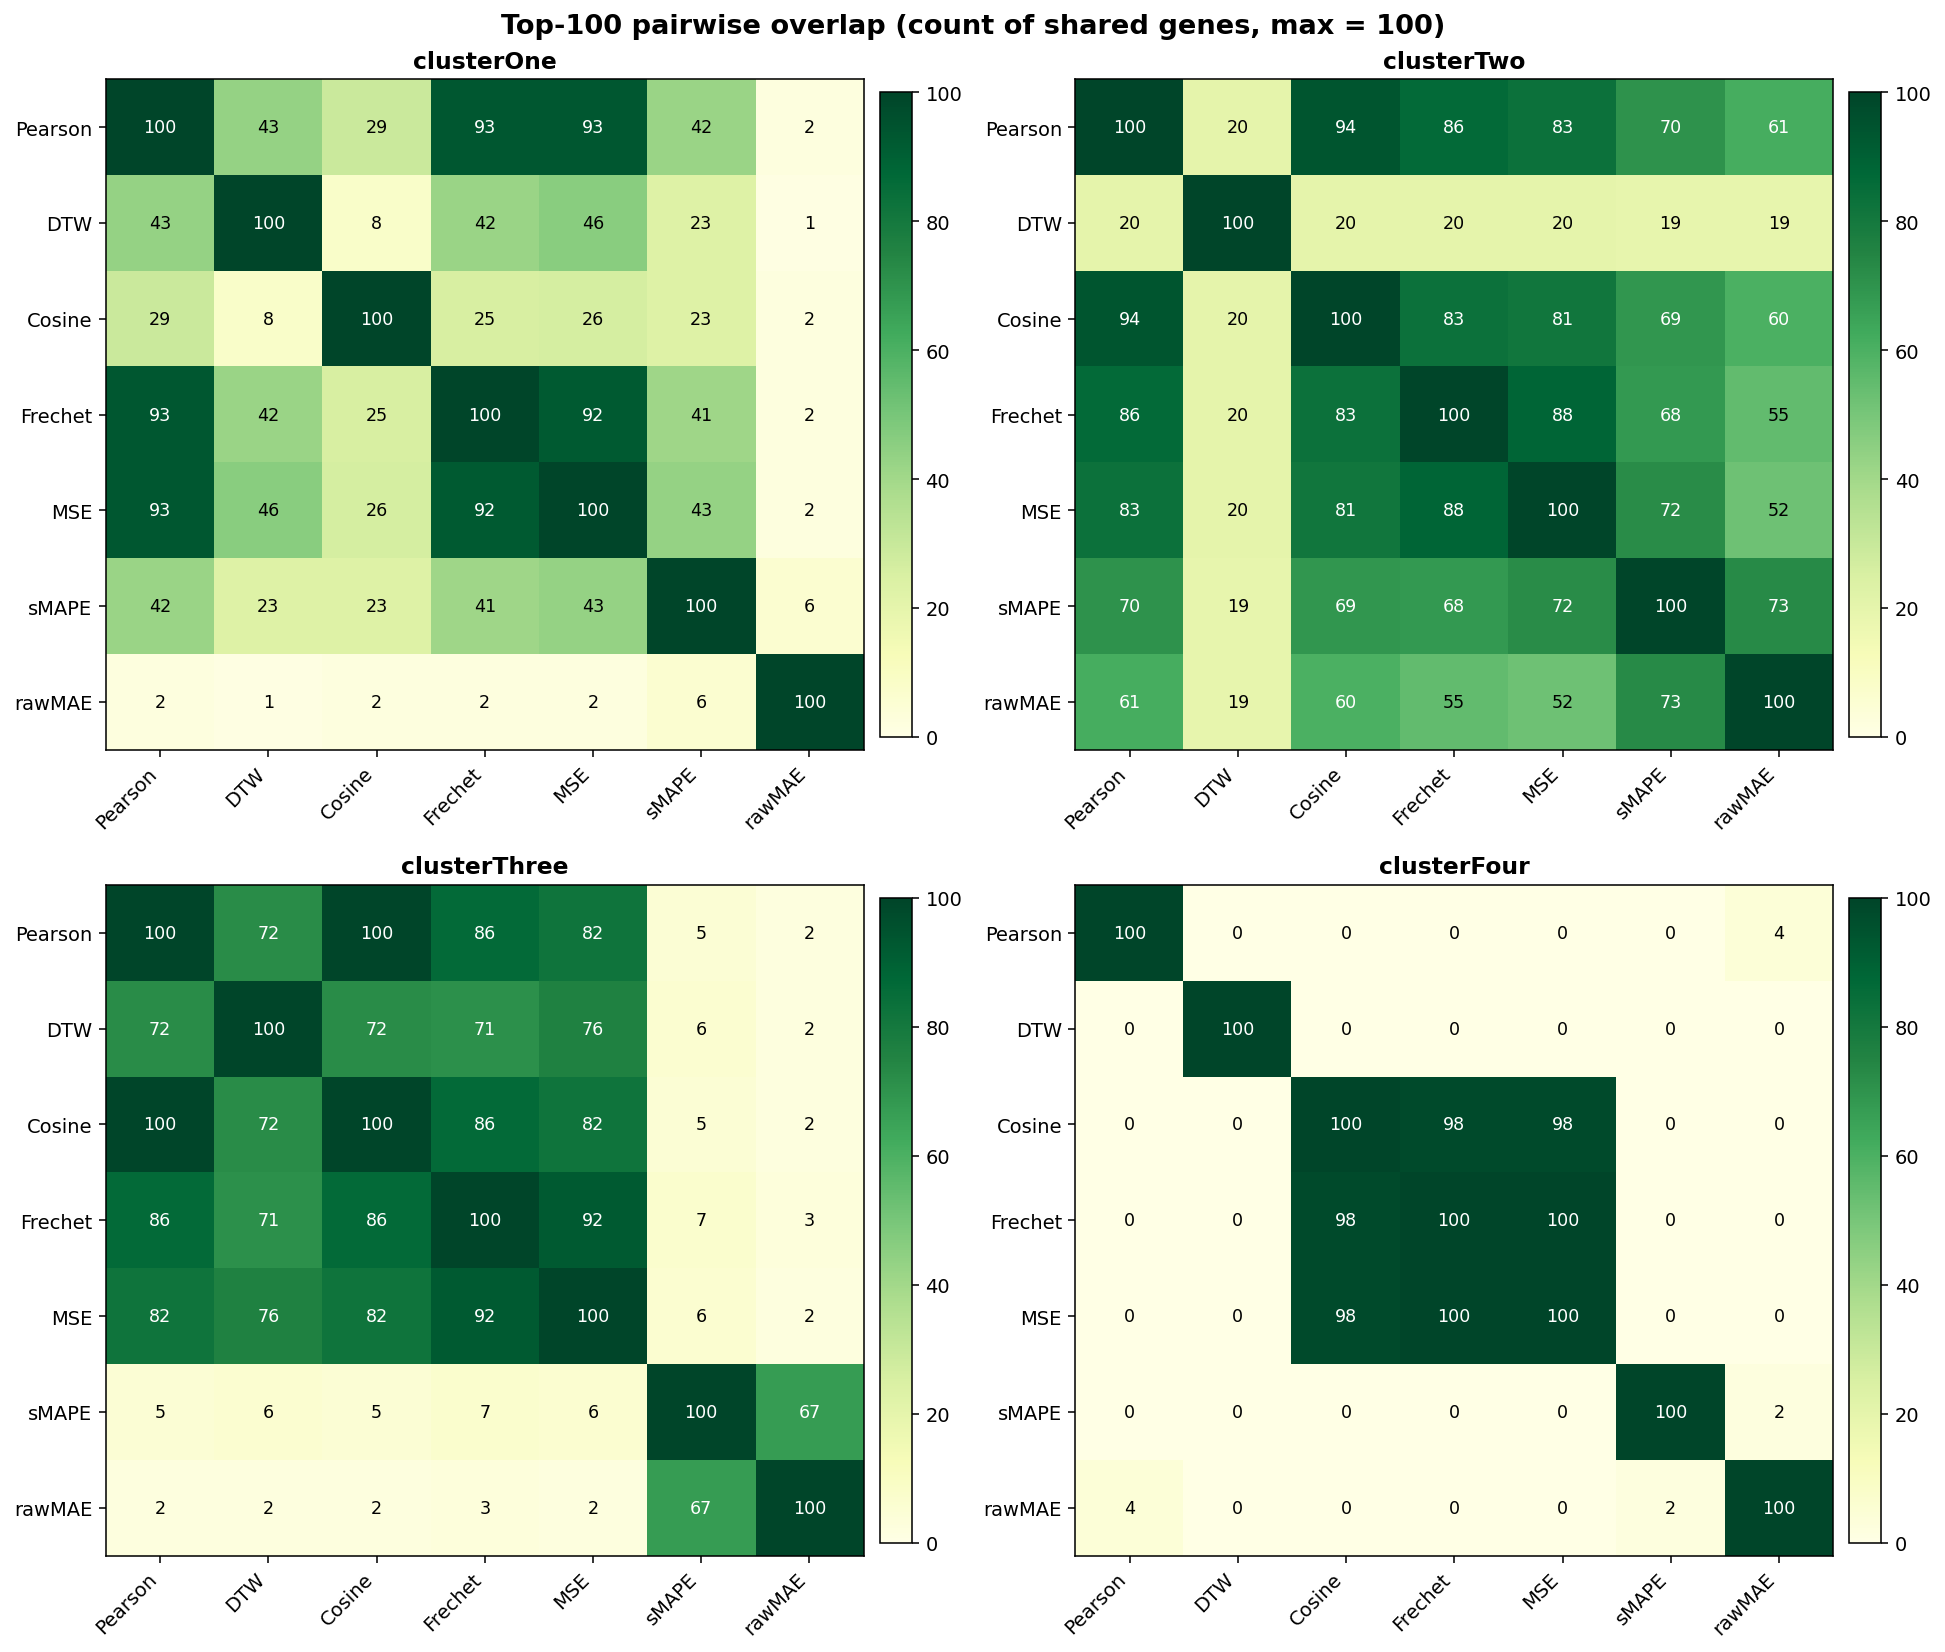
\includegraphics[height=0.78\textheight]{plots/top100_overlap_heatmap.png}
\\[0.1em]
\scriptsize
\textbf{clusterOne:} Pearson, Fr\'{e}chet, MSE share \textasciitilde 93/100 picks --- Pearson is the principled center of a tight consensus. \quad
\textbf{clusterTwo:} Pearson--Cosine flips to 94/100. \quad
\textbf{clusterThree:} Pearson--Cosine = 100/100 (V-shape unambiguous). \quad
\textbf{clusterFour:} Cosine/Fr\'{e}chet/MSE form a 98--100 spike-magnitude consensus; Pearson is alone (the only truly scale-invariant metric); rawMAE is alone (the only magnitude metric).
\end{frame}

% ------------------------------------------------------------------
\begin{frame}{Files Shipped to Ethan and Zihan}
\small
\begin{itemize}\itemsep0pt
  \item \texttt{deliverables/clusterOne\_ranking.csv} \quad (Pearson, 17{,}856 rows)
  \item \texttt{deliverables/clusterTwo\_ranking.csv} \quad (rawMAE, 17{,}856 rows)
  \item \texttt{deliverables/clusterThree\_ranking.csv} \quad (rawMAE, 17{,}856 rows)
  \item \texttt{deliverables/clusterFour\_ranking.csv} \quad (rawMAE, 17{,}856 rows)
  \item \texttt{deliverables/final\_gene\_lists.csv} \quad (combined, 71{,}424 rows)
\end{itemize}

\vspace{0.8em}
\textbf{Next:} pathway / GO enrichment on each cluster's top-N to see if the gene set hits a coherent biological process.
\end{frame}

\end{document}
